\chapter{Koncepció}

\section{Cél}
A szakdolgozatom célja egy webáruház létrehozása, amely első sorban numizmatikával foglalkozik, hogy ehhez a témához vonzódó felhasználók egyszerűen hozzá férhessenek olyan darabokhoz, amelyek esetleg hiányoznak a gyűjteményükből. Ezen felül egy olyan webáruhazát szeretnék létrehozni, amelyet kisebb átalakításokkal más webáruház létrehozásához is fel lehet használni. Emellett célom hogy az oldalt meglátogató felhasználók számára könnyen átlátható és egyszerűen használható legyen. Fejlesztői részről pedig egy olyan oldalt akarok létrehozni, amely a mai világban lévő komplikált webáruházak mellett is megállja a helyét.

\section{Kereslet a webáruházakra}
\large\textbf{Mi a webáruházak előnye?}

Az internet egyre széleskörűbb térhódításával a kereskedelem az utóbbi években hatalmas változáson ment és megy keresztül. Ennek következtében az emberek egyre nagyobb százaléka vásárol online. Ezt a folyamatot a 2020-ban kitörő koronavírus járvány még jobban felgyorsította. Mivel a kijárati tilalmak és egyéb korlátozások megnehezítették a bevásárlást. E-miatt néhány kisebb bolt szinte teljesen vagy csak részlegesen, de átállt a csak online való kereskedelemre.  Mivel az emberek egyre jobban megszokták, hogy otthonról rendelnek, és nem kell elmenniük az adott üzletbe és az adott boltnak is jobb. Mivel így az ország bármely pontjából vásárolhatnak tőle a vásárlók így egy sokkal tágabb csoporthoz el tudja juttatni a termékeit e mellett nem, kell az üzlet épületének fenntartásával foglalkozni a csak a raktárral, a csomagolással és a termékek kiszállításával. A kiszállítást viszont általában egy külsős cég felügyeli és intézi ezzel még kisebb teher alá téve az adott üzletet.

Azzal hogy már szinte minden ember zsebében  ott lapul az okostelefon, néhány kattintással már képesek az emberek vásárolni szinte bárhonnan a világból. Ez nagyban megkönnyítette az életüket mivel már nincs, szükség a bevásárlás előre való megtervezésének nem kell foglalkozni az üzemanyaggal vagy a forgalom miatt, ha szeretnének vásárolni. Elég csak a felhasználóknak bejelentkezniük az adott weblapra ahol vásárolni szeretnének és a termékek kiválasztása után leadni a rendelésüket.

Mivel a COVID alatt a boltokat csak időszakosan lehet használni vagy egy időszakban egy adott korosztálynak így az idősebb korosztályból is egyre többen elkezdtek érdeklődni az online vásárlás után, ami az e-kereskedelmet még széleskörűbbé tette.

\cite{20} 2020 júniusában és júliusában az IPC egy hazai e-kereskedelmi vásárlói felmérést végzett, amely számos kérdést tartalmazott a COVID-19-ről. A legfontosabb megállapítások a következők voltak:
\begin{itemize}
    \item A fogyasztók 52\%-a vásárolt többet online a hazai e-kiskereskedőktől a COVID-19 járvány idején, és a fogyasztók 21\%-a számolt be arról, hogy jelentősen többet vásárolt - ez a legmagasabb arány Portugáliában és az Egyesült Államokban volt.
    \item A fogyasztók 27\%-a vásárolt több élelmiszert online a COVID-19 világjárvány idején, és a legnagyobb növekedést az Egyesült Királyságban jelentették az online élelmiszervásárlás terén, ahol 30\%-kal többet vásároltak.
    \item A fogyasztók 49\%-a egyetértett azzal, hogy a COVID-19 miatt a jövőben többet fog online vásárolni.
\end{itemize}

\begin{figure}[h]
\centering
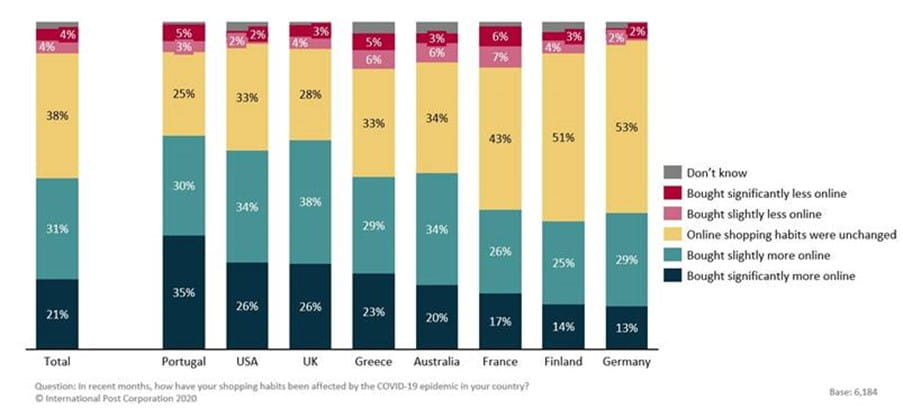
\includegraphics[scale=0.5]{images/IPC_velemeny_kutatas.jpg}
\caption{Kovid allati vásárlási szokásokról közvélemény kutatás.}
\label{fig:velemeny_kutatas}
\end{figure}

\section{Dropshipping}

\cite{21} A dropshipping az online áruházak egy olyan formája amelynél ha a vásárló rendel valamit az adott oldalról akkor nem a cég saját raktárából kapja meg a terméket. Hanem ez a cég csak egy harmadik féltől egy nagykereskedőtől vásárolja meg a terméket és azt közvetítti a vásárlónak. Így csak az értékesítést és a szállítást intézi az adott cég. 

\begin{figure}[h]
\centering
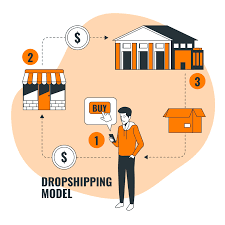
\includegraphics[scale=1.3]{images/dropshipping.png}
\caption{A dropshipping bemutatója \cite{22}}
\label{fig:dropshipping_modell}
\end{figure}

\subsection{Dropshipping előnyei}

\begin{itemize}
    \item \textbf{Kevesebb tőkét igényel és egyszerűbb beindítani}
    
Ez az egyik legnagyobb előnye mivel nincs szükség kezdő tőkére, hogy az ember egy ilyen webáruházat beindítson. Ez az miatt lehet, mert nem kell egy állandó árukészletet fen tartania egy raktár épületben, csak amikor rendelést kap, azt egy harmadik féltől kell megrendelnie. E miatt az értékesítő megspórolja a raktárépület bérlését, a csomagolási és szállítási költségeket, a készlet nyomon követését és fenntartását.

    \item \textbf{Alacsony fix költségek}
    
A fix készlet hiánya miatt sokat spórol a fenntartó, de nem csak ez az egyik fő indok, ami miatt olcsó. Nincs szüksége alkalmazottak felvevésére és telephely fenntartására ehhez a webáruház üzemeltetéseshez elég egy számítógép vagy laptop ritkábbik esetekben csak egy mobil telefon. E miatt a havi költségek igen minimálisak persze ez az összeg is növekedni fog ha az üzlet növekszik és ilyenkor már egy egyszerű mobiltelefon nem lesz elegendő. De továbbra is egy jóval olcsóbb megoldás mint más típusú webáruház üzemeltetése.

    \item \textbf{Rugalmas munkavégzési hely}
    
Ha az üzemeltető egy biztonságos és gyors internetkapcsolattal felszerelt helyen van akár onnan is dolgozhat. Egyetlen lényeg van, hogy tudjon kommunikálni a megrendelővel és a nagykereskedésekkel.

    \item \textbf{Óriási kínálat}
    
Mivel nem kell az árucikket előre megvásárolni így az üzletben óriási készletett kínálhat a vevőknek. ha egy nagykereskedő kínál egy terméket, azt a dropshipping üzlet is feltüntetheti minden extra költség nélkül.

    \item \textbf{Könnyedén skálázható}
    
Ha egy üzlethez az átlagosnál több megrendelés érkezik, azzal, jóval több munka van. De a dropshipping nagy előnye hogy a megrendelések nagy részét a nagykereskedések intézik.

\end{itemize}

\subsection{Dropshipping hátrányai}

\begin{itemize}
    \item Minimális profit
    
Ez a legnagyobb hátránya mivel könnyű belekezdeni, rengetegen bele is kezdenek így hatalmas a versenygés. Némely kereskedő a nagyon alacsony árakkal akarja magához vonzani a vevőket. Ez okból viszont nagyon alacsony lesz a profitjuk is, de ez az alacsony költségek miatt nem akkor probléma számukra. Mivel a vásárlókat csak az áru ára érdekli így még a kereskedőnek lehet jó profitja, ha sokan vásárolnak ott. Viszont a piac telítettsége miatt egyre kevésbé éri meg a dropshippinggel foglalkozni mivel annyira alacsony haszon folyik be belőle.

    \item Készletproblémák
    
Amikor egy hagyományos kereskedő a saját raktárkészletét kezeli, könnyedén nyomon követheti, hogy mennyi termék áll rendelkezésére. Viszont, ha valaki dropshipping kereskedőként a nagykereskedők raktárkészleteire támaszkodik, fennáll a veszélye annak, hogy a készletek gyorsan elfogynak. Ebben az esetben ugyanis minden más dropshipping kereskedő is ugyanezen készletekre hagyatkozik, ráadásul a hagyományos viszonteladóknak is időnként fel kell tölteniük saját készleteiket.

    \item Szállítási nehézségek
    
Általában egy dropshipping kereskedő több nagykereskedéssel dolgozik egyszerre így sokkal nehezebb nyomon követni a szállítási költségeket.

Például ha több terméket rendel és mindegyik terméket más nagykereskedőtől, akkor ott több szállítási költséget kell fizetni. Ezt a plusz összeget viszont nem szabad ráterhelni a vevőre mert úgy fogja érezni hogy túlvan árazva a szállítás.

\end{itemize}

